% Shared standalone design for the editable figure reconstructions.
\documentclass[tikz,border=5pt,10pt]{standalone}
\usepackage[T1]{fontenc}
\usepackage[utf8]{inputenc}
\usepackage{newpxtext,newpxmath}
\usepackage[scaled=.94]{sourcesanspro}
\usepackage{pgfplots}
\pgfplotsset{compat=1.18}
\usetikzlibrary{arrows.meta,calc,positioning,decorations.pathreplacing,
  decorations.markings,patterns,matrix,shapes.geometric,fit,backgrounds,
  intersections,angles,quotes}
\definecolor{ink}{HTML}{203746}
\definecolor{accent}{HTML}{146C78}
\definecolor{muted}{HTML}{667780}
\definecolor{signalred}{HTML}{B94B44}
\color{ink}
\tikzset{>=Latex,line width=.8pt,
  every node/.style={font=\small},
  axis/.style={->,draw=muted,line width=.5pt},
  guide/.style={draw=muted,dashed,line width=.45pt},
  curve/.style={draw=accent,line width=1pt},
  marker/.style={circle,fill=accent,inner sep=1.5pt},
  labelbox/.style={fill=white,inner sep=2pt}}

\begin{document}
\begin{tikzpicture}
\path[use as bounding box] (-5.5,-2.8) rectangle (5.5,3.2);\draw[accent!22,line width=.55pt] (0,0) ellipse (0.6 and 0.2683281572999747);
\draw[accent!22,line width=.55pt] (0,0) ellipse (1.2 and 0.5366563145999494);
\draw[accent!22,line width=.55pt] (0,0) ellipse (2.2 and 0.9838699100999075);
\draw[accent!22,line width=.55pt] (0,0) ellipse (3.6 and 1.6099689437998486);
\draw[->,accent,line width=1pt] (3.0000,1.1000)--(2.2652,-0.2471);
\draw[->,accent,line width=1pt] (2.2652,-0.2471)--(1.0837,0.3974);
\draw[->,accent,line width=1pt] (1.0837,0.3974)--(0.8183,-0.0893);
\draw[->,accent,line width=1pt] (0.8183,-0.0893)--(0.3915,0.1435);
\draw[->,accent,line width=1pt] (0.3915,0.1435)--(0.2956,-0.0322);
\draw[accent,line width=.65pt] (0.2956,-0.0322)--(0.1414,0.0518)--(0.1068,-0.0116)--(0.0511,0.0187)--(0.0386,-0.0042);
\fill[ink] (3.0000,1.1000) circle (1.4pt);
\node[above right] at (3.0000,1.1000) {$x_0$};
\fill[ink] (2.2652,-0.2471) circle (1.4pt);
\node[below right] at (2.2652,-0.2471) {$x_1$};
\fill[ink] (1.0837,0.3974) circle (1.4pt);
\node[above left] at (1.0837,0.3974) {$x_2$};
\fill[ink] (0.8183,-0.0893) circle (1.4pt);
\fill[ink] (0.3915,0.1435) circle (1.4pt);
\fill[ink] (0.2956,-0.0322) circle (1.4pt);
\fill[ink] (0.1414,0.0518) circle (1.4pt);
\fill[ink] (0.1068,-0.0116) circle (1.4pt);
\fill[ink] (0.0511,0.0187) circle (1.4pt);
\fill[ink] (0.0386,-0.0042) circle (1.4pt);
\draw[signalred,line width=.7pt] (2.3610,-0.0715)--(2.1854,0.0242)--(2.0896,-0.1513);
\fill[signalred] (0,0) circle (1.7pt) node[below left] {$x^\star$};

\node at (0,2.65) {$\tau_k\in\underset{\tau\geq0}{\operatorname{argmin}}\ f(x_k-\tau\nabla f(x_k))$};
\node at (0,-2.0) {$\langle\nabla f(x_k),\nabla f(x_{k+1})\rangle=0$};
\node[font=\footnotesize] at (0,-2.55) {$f(x)=\tfrac12(x_1^2+5x_2^2)$};
\end{tikzpicture}
\end{document}
